%%%%%%%%%%%%%%%%%%%%%%%%%%%%%%%%%%%%%%%%%%%%%%%%%%%%%%%%%%
%%
%%  LOD-Postface.tex
%%  Postface: The Beginning of Diffeological Spaces
%%
%%%%%%%%%%%%%%%%%%%%%%%%%%%%%%%%%%%%%%%%%%%%%%%%%%%%%%%%%%

\backmatter

\cleardoublepage
\chapter*{Postface: The Beginning of Diffeological Spaces}
\setcounter{footnote}{0}

%%%%%%%%%%%%%%%%%%%%%%%%%%%%%%%%%%%%%%%%%%%%%%%%%%%%%%%%%%
%%
%% MARK: Content
%%
%%%%%%%%%%%%%%%%%%%%%%%%%%%%%%%%%%%%%%%%%%%%%%%%%%%%%%%%%%

The word ``diffeologies'' first appears in Souriau's paper {\em Groupes différentiels},
the text of a talk presented at a conference in Salamanca in 1979 and published in 1980 \cite{Sou80}.
In this article,
a ``difféologie'' refers to an abstract structure used to define exclusively what Souriau called ``groupes différentiels''.
It is defined by five axioms,
the last two of which relate specifically to the group structure.
Although Souriau could have removed those last two axioms and thus defined the general concept of ``espaces différentiels'',
he did not do so in this article.
His ``difféologies'' remained, at that time, tied to groups.

The general concept of ``espace différentiel'',
as it would later emerge,
is in fact absent from this 1980 paper.
It would take three years,
and some unexpected developments,
for this notion to appear in its own right.

Souriau's focus on groups is understandable when we know that
he was looking then for a renewal of his method of quantization
through the Gelfand-Naimark-Segal construction,
using positive-definite functions on a given group of symmetries.
But because the Dirac program requires representing
the whole group of symplectomorphisms,
Souriau had to leave the category he used to work in
--- that of finite-dimensional Lie groups ---
to deal with the huge infinite-dimensional group of all symplectomorphisms.
Instead of paying tribute to the thick theory of topological groups,
he preferred to build his own light category of
``groupes différentiels'', retaining just the minimal properties he needed.
That gave his 1980 paper.

For a couple of years Souriau continued to work on this approach.
At the time,
Paul Donato, also a student of Souriau,
was interested in this new concept.
He wrote an essay in 1981 on the fundamental group of a manifold
through its group of diffeomorphisms \cite{Don81},
and later made this the subject of his 1984 dissertation \cite{Don84}.
On my side, I was working on something very different ---
the classification of $\SO(3)$ symplectic manifolds ---
and these ``groupes différentiels'' did not speak to me that much.

The next step came in June 1983 during a conference in Lyon,
where Souriau was invited to talk, and Paul and I were attending.
At the same conference we heard talks about what we later called ``irrational tori'',
quotients of the $2$-torus by an irrational line.
Alain Connes had already introduced his non-commutative geometry to study these objects,
which escape traditional differential geometry.

Paul had already developed tools to compute the fundamental group of a coset of a ``groupe différentiel''
and even to build its universal covering in some cases.
Intrigued,
we decided then to investigate the irrational torus from this point of view.
We computed its fundamental group and universal covering,
and were amazed to find that two irrational numbers give diffeomorphic tori
if and only if they are conjugate modulo $\GL(2,\ZZ)$.
We were even more surprised by the computation of the connected components of the group of diffeomorphisms,
which distinguishes quadratic from non-quadratic irrationals.

We published these results in a preprint titled
``Exemple de groupes différentiels : flots irrationnels sur le tore'',
in July 1983 \cite{DI83}.
As far as I know, it is in this preprint that,
for the first time,
the expression ``espace différentiel'' was used.
It appears between quotes,
on the second page (page 112 of the Preprint CPT-83/P.1524),
as shown in the detail of the facsimile displayed in Figure \ref{fig:first-espace-differentiel}.

%\begin{quote}\n
%Les applications différentiables de ${\mathcal \Torus_\alpha}$ à valeurs dans un ``espace différentiel'' $E$,\n
%sont les applications $\varphi : {\mathcal \Torus_\alpha} \to E$ telles que pour tout $f$ élément de $D(\mathbf{R}^n,\mathcal \Torus_\alpha)$,\n
% $\varphi \circ f$ est un élément de $D(\mathbf{R}^n,E)$.\n
% En particulier les difféomorphismes de $\mathcal{T}_\alpha$ à $E$ sont les bijections bi-différentiables.\n
%\end{quote}\n

\begin{figure}[htbp]
\centering
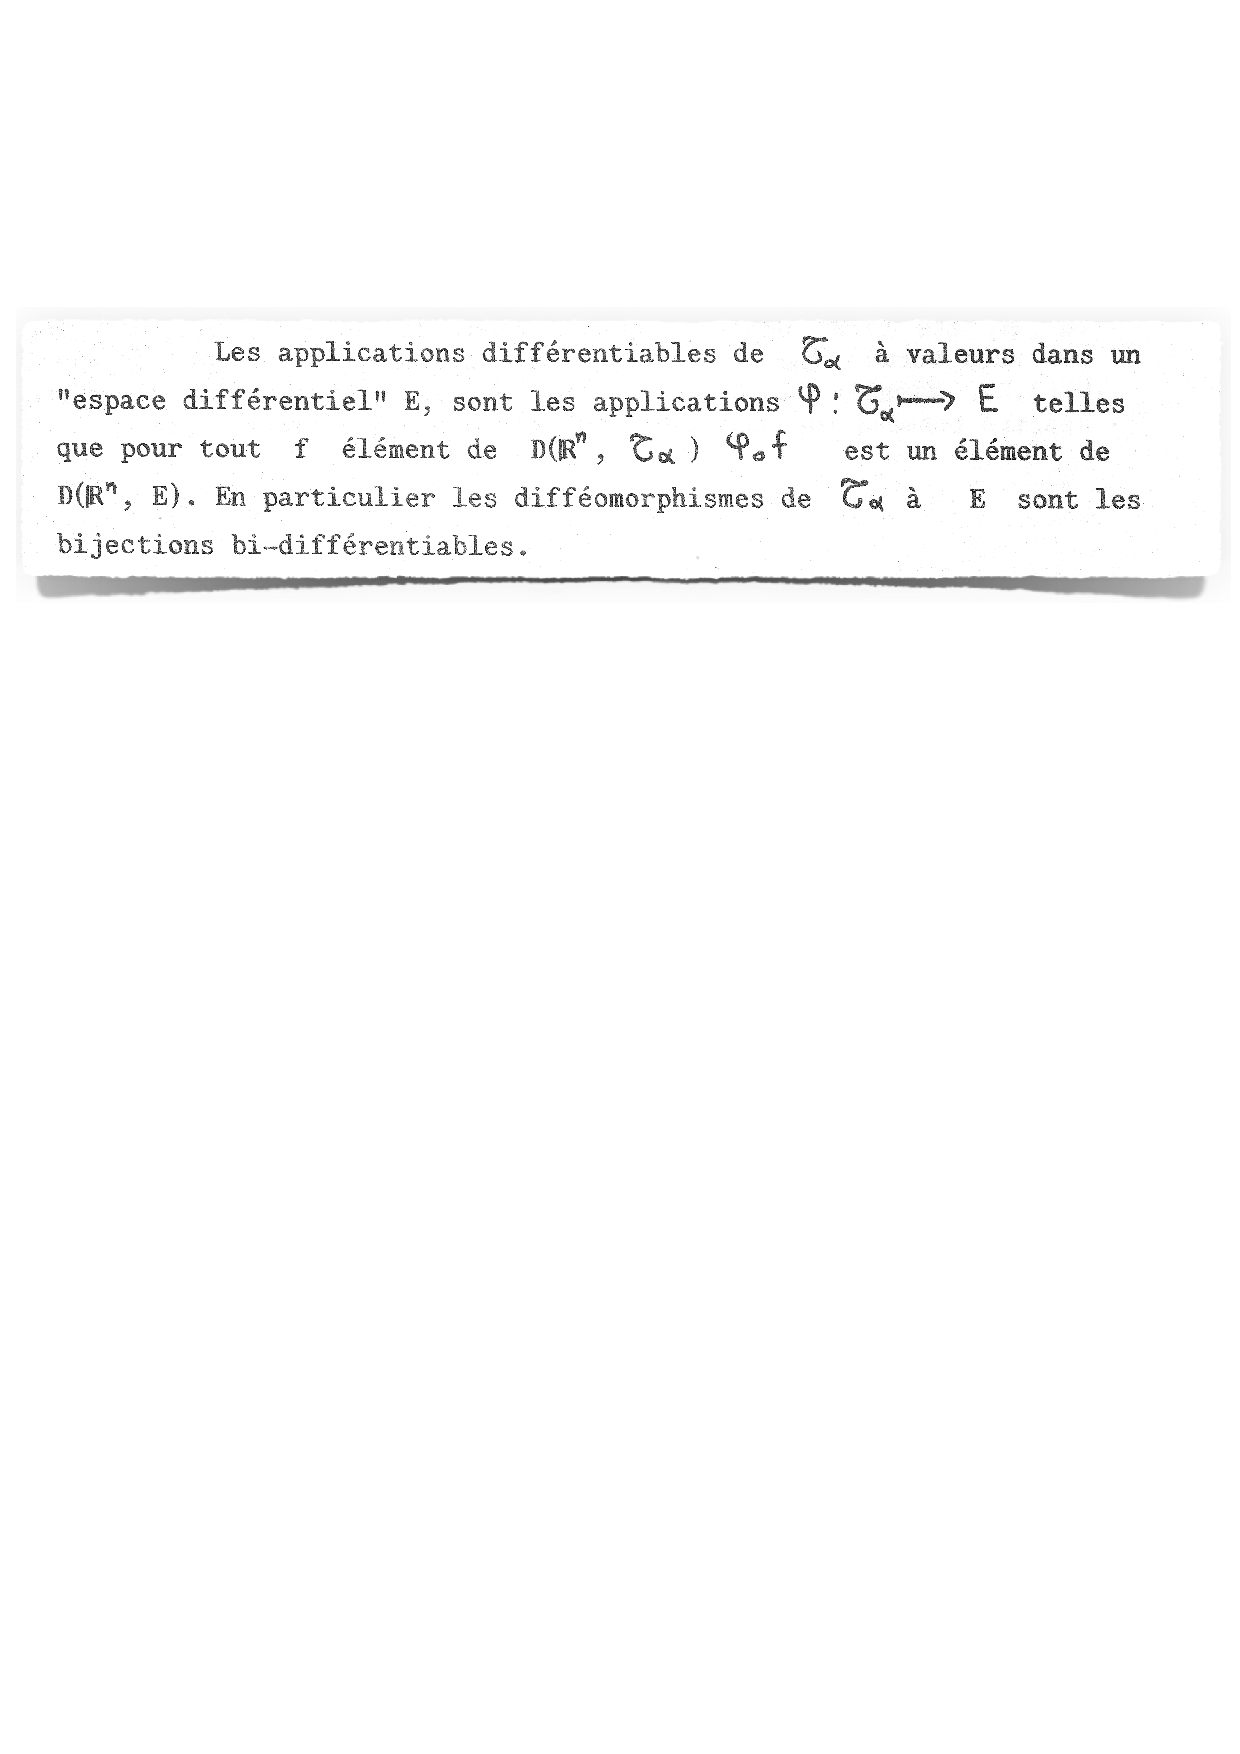
\includegraphics[width=\textwidth]{Figures/facsimile-page112.pdf}
\caption{Detail of page 112 from the July 1983 preprint \cite{DI83},
showing the first written occurrence of ``espace différentiel'' (in quotes).}
\label{fig:first-espace-differentiel}
\end{figure}

This conceptual step
--- defining a category of spaces with a plot-based smooth structure ---
was essential for building the broader theory of diffeology as it is known today.
However, the preprint contained no formal axiomatic definition of such spaces.
It used the notion operationally, as a working tool.

I remember lively discussions about the need for a general definition.
One summer day that year, the whole team was together at the cafeteria of Luminy campus for a coffee break.
Paul and I insisted on a formal definition of differential spaces,
while Souriau resisted, thinking such generality was unnecessary for his quantization program.
But Paul needed a coherent framework of ``espaces différentiels'' for his dissertation,
and I had begun to think about generalizing our results through homotopy and fiber bundles,
which also required a solid foundation.
Under this pressure, Souriau changed his mind.
A few weeks later, in October 1983, he included the formal (axiomatic) definition of ``espace différentiel''
in his preprint ``Groupes différentiels et physique mathématique'' \cite{Sou84}.

\iffalse
Had diffeology remained confined to Souriau's original ``groupes différentiels'',
the concept of ``espace différentiel'' --- the three-axiom definition that underpins the theory today ---
might never have been extracted.
And without that generalization,
the Wire Plane $\cW$,
which is not a group,
not homogeneous,
not a quotient of a group,
would have remained invisible.
The Boman Paradox,
which reveals the limits of the radical Kleinian--Souriau claim that ``le groupe est la géométrie'',
depends crucially on this broader notion of space.
Thus,
the very generality that Paul and I urged upon Souriau in 1983
--- against his initial reluctance ---
is what ultimately provided the counterexample to his own philosophical stance.
The arrow of definition is irreversible:
the space determines the group,
but the group,
even as a diffeological group,
does not determine the space.

Of course,
one could artificially equip the set $\Diff(\RR^2)$ with the functional diffeology of the wire plane,
but that would be an arbitrary construction.
What makes the situation natural is that this diffeology comes from the geometry of $\cW$ itself,
just as the standard diffeology on $\Diff(\RR^2)$ comes from the geometry of $\RR^2$.
The space determines the group,
not the other way around.
The fact that two different spaces produce two different diffeological group structures
on the same abstract set is not a trick;
it is a genuine geometric phenomenon.
It reveals that the geometry of a space is encoded in the diffeology of its symmetry group,
but that diffeology cannot be recovered from the abstract group alone.
\fi

That is how the diffeology of spaces was born.
It took from 1980 to 1983 to move from groups to spaces, and from five axioms to three.
If the first implicit use of ``espace différentiel'' appears in our July 1983 preprint,
the definitive axiomatic formulation is due to Souriau,
prompted by the needs that Paul and I had brought to light.
The theory then became what it is today.

\medskip
\textbf{Note on the 1983 preprint.}
The preprint ``Exemple de groupes différentiels : flots irrationnels sur le tore'' (July 1983, CPT-83/P.1524) is preserved in the ``Diffeology-Archives" repository.
at the following URL.%
\footnote{Available at: \\ \url{https://github.com/p-i-z/Diffeology-Archives/blob/main/Papers/1983-Flots-Irrationnels-sur-le-Tore/DIZ83-preprint-1983.pdf}}
The page 112 contains the first known use of the term ``espace différentiel'' in the diffeological literature,
albeit without a formal axiomatic definition.
That definition would appear a few months later in Souriau's October 1983 preprint.
Truth be told,
I long assumed Souriau had forgotten to cite us --- a habit of his,
as is well known.
But years later I discovered,
to my surprise,
that he did cite our July 1983 preprint in note 9 of his October 1983 paper \cite{Sou84}.
How badly I had judged my master...
\markboth{}{}
